\documentclass[a4paper,fleqn]{cas-sc}   %{article}
%remove ORCID footnote
\renewcommand{\printorcid}{}


%\usepackage{natbib}
% cas-common.sty references \bibsep (a natbib length) even when natbib is not loaded.
% Declaring it here prevents the "Undefined control sequence" error at \begin{document}.
\newlength{\bibsep}
\usepackage{float}
\usepackage{pdflscape}
\usepackage{array}
\usepackage{multirow}
\usepackage{booktabs}
\usepackage{longtable}
\usepackage{caption}
\captionsetup[longtable]{labelfont=bf,labelsep=newline,singlelinecheck=false,justification=raggedright}
\usepackage{adjustbox}
\usepackage[style=authoryear-icomp,
uniquelist=false,
maxnames=2,
minnames=1,
maxbibnames=99,
    backend=biber, giveninits=true,
    ibidtracker=false,
    uniquename=false,
    natbib=true]{biblatex}

\addbibresource{../battery_paper/DCE_lit_review.bib}
\addbibresource{../battery_paper/Used EV.bib}
\addbibresource{../battery_paper/EV battery.bib}
% \DeclareNameAlias{default}{family-given}

\usepackage{hyperref}
\usepackage{graphicx}

% Force floats to appear where inserted, not deferred to end of document.
% Use [H] specifier on every \begin{figure} and \begin{table}.
% The parameters below allow LaTeX to place floats very liberally.
\renewcommand{\topfraction}{0.99}
\renewcommand{\bottomfraction}{0.99}
\renewcommand{\textfraction}{0.01}
\renewcommand{\floatpagefraction}{0.99}
\setcounter{topnumber}{20}
\setcounter{bottomnumber}{20}
\setcounter{totalnumber}{40}

% add line number
\usepackage{lineno}
\pagewiselinenumbers

% remove the "preprint"
\ExplSyntaxOn \cs_gset:Npn \__first_footerline: { \group_begin: \small \sffamily \__short_authors: \group_end: } \ExplSyntaxOff

% remove "of X" from footer — redefine source functions then re-apply page style
\ExplSyntaxOn
\cs_gset:Npn \__first_foot: {
  \parbox[t]{\textwidth}{
    \rule{\textwidth}{.2pt}\\
    \__first_footerline: \hfill Page~\thepage
  }
}
\cs_gset:Npn \__cas_foot: {
  \parbox[t]{\textwidth}{
    \rule{\textwidth}{.2pt}\\
    \sffamily\small \__first_footerline: \hfill Page~\thepage
  }
}
\ExplSyntaxOff
\AtBeginDocument{\pagestyle{cas}}


% suppress abstract section
\renewenvironment{abstract}{}{}
\renewcommand{\abstractname}{}

\shortauthors{}

%%%Author macros
\def\tsc#1{\csdef{#1}{\textsc{\lowercase{#1}}\xspace}}
\tsc{WGM}
\tsc{QE}
\tsc{EP}
\tsc{PMS}
\tsc{BEC}
\tsc{DE}
%%%


\begin{document}
\let\WriteBookmarks\relax
\def\floatpagepagefraction{1}
\def\textpagefraction{.001}
\shorttitle{}

\title [mode = title]{Consumer Valuation of Battery Health Information in Used Electric Vehicle Markets: A Discrete Choice Experiment
}


\author[1]{Xiatian {Iogansen}}
\fnmark[1]

\author[1]{Zain {Hoda}}
\fnmark[2]

\author[1]{John P. {Helveston}}
\fnmark[3]

\address[1]{Department of Engineering Management and Systems Engineering, George Washington University, Washington D.C., USA}



\fntext[fn1]{xiatian.iogansen@gwu.edu, https://orcid.org/0000-0002-4851-1323}
\fntext[fn2]{zain.hoda@gwu.edu}
\fntext[fn3]{jph@gwu.edu, https://orcid.org/0000-0002-2657-9191}


\maketitle
\renewcommand{\baselinestretch}{1}\normalsize
\section{Introduction}
\label{section:intro}

The used vehicle market plays a central role in U.S. automobile ownership: used vehicle transactions now account for roughly 70\% of all passenger vehicle purchases and are projected to grow steadily through the coming decade \parencite{marketresearchfutureUnitedStatesUsed2025}. As battery electric vehicles (BEVs) continue to penetrate the new car market, an increasing number of BEVs are entering the secondary market. Despite this momentum, consumer hesitation toward used BEVs remains pronounced. \textcite{fernandesUSUnderstandingConsumer2023} indicates that 52\% of U.S. adults are unlikely to consider purchasing a used EV. Consumers frequently cite uncertainty about vehicle and battery condition (41\%) and concerns about reliability relative to new EVs (23\%) as primary barriers. This gap between perceived and actual risk points to a fundamental information asymmetry: buyers lack information and knowledge about the battery at the point of sale, which represents up to 30\% of a used BEV's value \parencite{boudwayBatteriesElectricCars2020}.

Unlike conventional vehicles, where odometer reading and vehicle age serve as reasonable proxies for overall wear, unique attributes of the used BEVs, including battery degradation, battery refurbishment, warranty coverage, increase the uncertainty for consumers. This paper asks how consumers value battery health information among used BEVs and how preferences vary across consumer segments. We address these questions using a discrete choice experiment (DCE) in an online survey administered to a national U.S. sample of 2,916 adults who reported an intention to purchase a used car or SUV within the next two years. The DCE presents respondents with repeated choices among hypothetical used BEVs that vary in mileage, purchase price, electric range, battery degradation rate, and battery refurbishment history. 

We estimate a latent class choice model (LCCM) which reveals six distinct consumer segments that differ markedly in their sensitivity to battery quality signals, price, and the no-choice option. Vehicles with documented performance indicators and battery health information represent a material pricing premium opportunity with the majority of the market. To our knowledge, this study provides the first WTP estimates for battery health information in the U.S. used BEV market. These findings carry direct implications for used vehicle dealers, OEMs, and certification service providers seeking to develop market infrastructure for used BEVs.

\section{Survey Design, Data Collection and Modeling Approach}

Each respondent completes six repeated choice tasks. Prior to the choice tasks, respondents are shown descriptions of all attributes (see Table~\ref{table:dce_attributes}). During the DCE design phase, we used range at the time of manufacture (Year~0) and an annual degradation rate to characterize battery condition. To improve comprehension for respondents, we transformed these underlying design parameters and presented range and SOH at Year~3 (the current purchase date) and Year~8 (five years after purchase).Figure~\ref{fig:battery_dce} shows an example choice task, in which respondents select among three used BEVs or a ``None of the above'' option. 

In addition to the DCE, the survey collects information across three broader topic areas, including their current household vehicle fleet and their future vehicle purchasing intention, their knowledge, attitudes, and perceptions regarding EVs and battery technology, as well as demographic information.


\begin{table}[pos=H]
\caption{BEV choice experiment attributes and levels.}
\label{table:dce_attributes}
\begin{adjustbox}{width=\textwidth, center}
{\renewcommand{\arraystretch}{1.4}
\begin{tabular}{p{3.2cm} p{4.8cm} p{3cm} p{3cm} p{3cm} p{3cm}}
\toprule
\multirow{2}{*}{\textbf{Attribute}} & \multirow{2}{*}{\textbf{Definition}} & \multicolumn{4}{c}{\textbf{Levels}} \\
\cmidrule(lr){3-6}
 & & \textbf{Low-budget} \newline ($\leq$\$20K) Car & \textbf{High-budget} \newline ($>$\$20K) Car & \textbf{Low-budget} \newline ($\leq$\$20K) SUV & \textbf{High-budget} \newline ($>$\$20K) SUV \\
\midrule
Mileage & The total number of miles a vehicle has traveled since manufacture. & \multicolumn{4}{p{12.5cm}}{15,000--60,000 miles, in increments of 500 miles.} \\
\addlinespace[4pt]
Battery refurbishment history & The repair or replacement work that has been performed on the vehicle's main battery pack. & \multicolumn{4}{p{12.5cm}}{%
  \textit{(1) Original:} The battery remains in its factory-original condition with no repairs or replacements.\newline
  \textit{(2) Some battery cells replaced:} A portion of the battery cells has been replaced to address performance issues or extend battery life; the remaining cells are original.\newline
  \textit{(3) Entire battery pack replaced:} The full battery pack has been replaced with a new, refurbished, or used pack, typically after battery performance declined below a specified threshold.} \\
\addlinespace[4pt]
Electric range at delivery (Year 0) & The maximum distance the vehicle can travel on a full battery charge under typical driving conditions, as rated at the time of manufacture. & 50--150 miles \newline (50-mile increments) & 100--250 miles \newline (50-mile increments) & 150--250 miles \newline (50-mile increments) & 200--350 miles \newline (50-mile increments) \\
\addlinespace[4pt]
Battery annual degradation rate and state of health (SOH) & The average annual percentage loss in electric range and battery SOH. The remaining range and SOH at Year 3 (current) and Year 8 (five years from purchase) are derived from this rate. & \multicolumn{4}{p{12.5cm}}{1\%--8\%, in increments of 1\%.} \\
\addlinespace[4pt]
Purchase price & The total cost of the vehicle in dollars, including down payment, monthly payments, taxes, and fees. & \$10,000--\$20,000 \newline (\$2,000 increments) & \$20,000--\$40,000 \newline (\$5,000 increments) & \$15,000--\$25,000 \newline (\$2,000 increments) & \$25,000--\$45,000 \newline (\$5,000 increments) \\
\bottomrule
\end{tabular}}
\end{adjustbox}
\end{table}

\begin{figure}[pos=H]
    \centering
    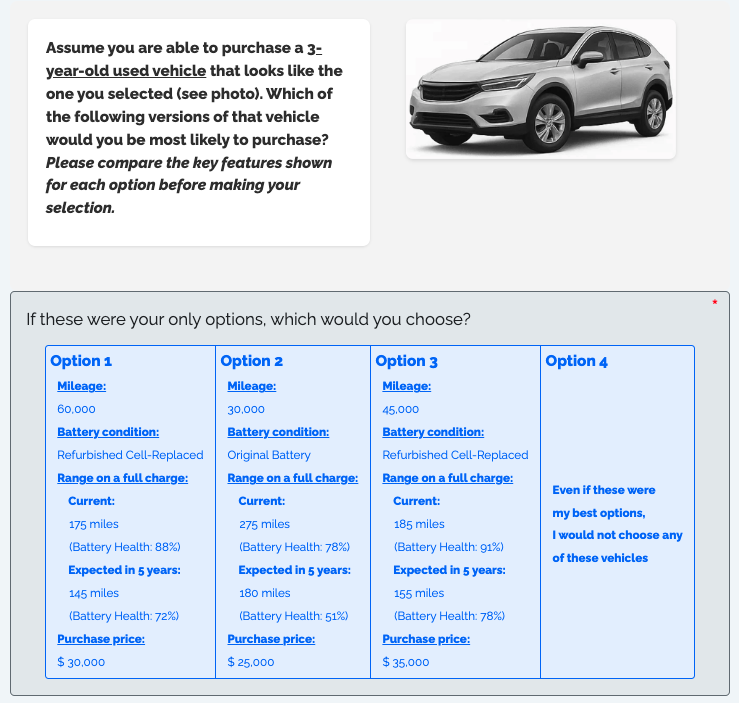
\includegraphics[width=0.7\textwidth]{../../code/output/images/battery_analysis/battery-1.png}
    \caption{Example of a choice experiment.}
    \label{fig:battery_dce}
\end{figure}




To identify discrete consumer segments that differ systematically in their battery quality sensitivity and price responsiveness, we estimate a Latent Class Choice Model (LCCM). The LCCM assumes that individuals can be assigned to a finite number of unobserved groups (classes) within which preferences are homogeneous, but across which they differ. The LCCM consists of two simultaneously estimated components (Figure~\ref{fig:model_framework}). The \textit{class membership model} assigns each respondent probabilistically to a latent class as a function of observable individual characteristics. The \textit{class-specific choice model} then estimates the conditional probability of each vehicle choice within each class. In addition, a set of \textit{inactive indicators}---attitudinal and behavioral variables excluded from estimation due to potential collinearity or theoretical considerations---are used to further characterize the classes descriptively after estimation. The formal model structure follows the notation of \textcite{chenExploringTouristPreference2023}.

A key output of the LCCM is class-specific WTP for each BEV attribute. Under the assumption that the marginal utility of price is negative and constant across alternatives, WTP for a given attribute in a given class is computed as the negative ratio of the attribute coefficient to the price coefficient. This represents the maximum dollar amount a representative respondent in that class would pay, or accept as compensation, for a one-unit change in the attribute, holding all other attributes constant.


\begin{figure}[pos=H]
    \centering
    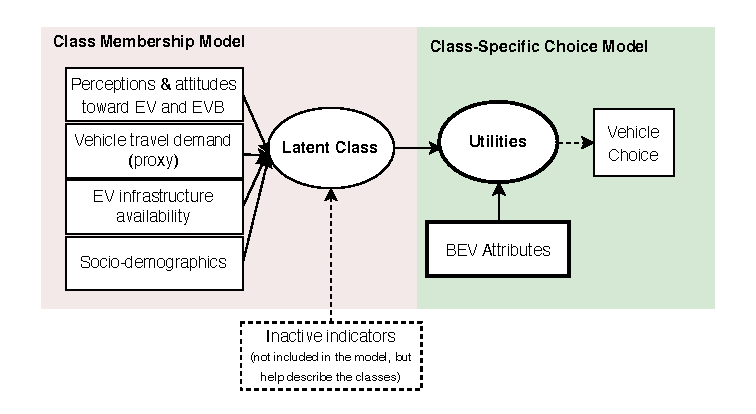
\includegraphics[width=0.8\textwidth]{../../code/output/images/battery_analysis/latent_class/model_framework.pdf}
    \caption{LCCM model framework.}
    \label{fig:model_framework}
\end{figure}

\section{Results and Discussion}
\label{section:results}

\noindent\textbf{Class 1: Opt-Out Dominant, BEV-Skeptical Consumers ($n$=252, 8.7\%).}\\
Class~1 is opt-out dominant. As a result, most WTP estimates for vehicle attributes are statistically indistinguishable from zero, with the exception of a moderate disutility for range loss in the 5--12\% segment (\$1.6k* per percentage point) and significant penalties for both pack replacement (\$6.4k*) and cell replacement (\$7.3k*).

Class~1 represents consumers who are not yet viable participants in the used BEV market. The majority (70.4\%) strongly disagree that they are likely to purchase a used BEV. They are the oldest class on average (47.1 years old), the least risk-tolerant (24.0\%), and with the least environmental awareness. Their household fleets are almost exclusively internal combustion engine vehicles (ICEVs), with 89.3\% of households reporting no EVs and 93.3\% driving an ICEV as their primary vehicle. EV-related knowledge is low (68.5\% correctly answer the EV knowledge question; only 10.6\% are aware of federal EV subsidies), while range anxiety is the highest of any class (87.2\%). Attitudes toward refurbished batteries are notably negative. Infrastructure readiness is also limited: only 32.8\% have home electrical outlet access, and only 24.7\% report a neighbor who owns or leases a BEV or PHEV.

\medskip

\noindent\textbf{Class 3: Range-Focused, EV-Engaged Consumers ($n$=485, 16.6\%).}\\
Class~3 stands in sharp contrast to Class~1, representing the most EV-engaged segment in the sample. It is distinguished by an exceptionally high WTP for range: \$38.7k*** per 100 miles for vehicles with 40--130 miles of range, declining to \$20.8k*** (130--200 miles) and \$25.5k*** (200+ miles). Their range loss aversion is moderate and uniformly significant across all degradation segments (\$0.9k***, \$0.7k***, \$0.5k***). Notably, WTP for refurbishment is negligible and statistically insignificant, suggesting that this class focuses more on current and future performance rather than battery refuishment history.

They hold the most favorable attitudes toward refurbished batteries (65.5\% agree they are environmentally beneficial; 35.5\% disagree that they are functionally inferior). Their households show the lowest rate of ICEV-only composition (74.1\%), and they are the most likely class to prefer a car over an SUV (57.2\%). They have the highest electrical outlet access (57.5\%), along with the strongest EV knowledge (81.1\%) and subsidy awareness (31.9\%). They have the highest household income (\$97.1k), report the highest employment rate (71.5\%), are the most risk-tolerant of all classes (39.0\% agree with a risk-taking characterization).

\medskip

\noindent\textbf{Class 2: Battery Health Attentives ($n$=661, 22.7\%).}\\
Class~2 is the largest class, which is uniquely defined by their battery health sensitivity. Range loss aversion is the highest across classes and uniform at approximately \$2.3k*** per percentage point across all three degradation segments. Both refurbishment types also generate meaningful disutility (\$2.7k* for pack replacement; \$3.8k** for cell replacement). Their range WTP is consistent across the three piecewise segments (\$4.6k, \$4.6k, and \$5.3k**), indicating a steady marginal valuation of additional range without a strong threshold effect though only the highest tier reaches statistical significance.

Members of Class~2 have an average household income of \$91.3k and are relatively young (36.5 years). They demonstrate above-average EV knowledge (76.2\%), moderate electrical outlet access (46.0\%), and a high rate of EV-owning neighbors (43.5\%). This class represents well-informed consumers are not necessarily purchasing range; rather, they are purchasing battery reliability at point of sale and protection against future performance loss.

\medskip

\noindent\textbf{Class 5: Multi-Attribute Maximizers ($n$=606, 20.8\%).}\\
Class~5 exhibits statistically significant evaluations across all vehicle attributes. This class places a high premium on crossing the minimum viable range threshold, with still-substantial but diminishing WTP at higher range levels (\$11.8k***, \$9.5k***, \$9.5k***). Range loss aversion is uniformly significant at \$0.8k*** per percentage point across the lower two degradation segments, tapering at the highest degradation level (\$0.4k*). Refurbishment disutility is among the highest of the attribute-sensitive classes (\$5.8k*** for pack replacement; \$6.1k*** for cell replacement).

What further distinguishes Class~5 is its opt-out pattern: only 5.2\% of members never opt out. Class~5 members exhibit high range anxiety (83.4\%) and are particularly averse to battery refurbishment (only 18.8\% disagree that refurbished batteries are functionally inferior). They also report average household incomes (\$86.9k) and lower risk tolerance. These characteristics lead them to make cautious, holistic evaluations across all vehicle attributes simultaneously. When a choice set presents no option that reach minimal quality threshold across all dimensions at once, respondents in this class choose to opt out rather than settle for the least-bad alternative.

\medskip

\noindent\textbf{Class 6: Budget-constrained, Low-WTP Consumers ($n$=373, 12.8\%)}\\
Class~6 has the largest price coefficient in absolute value ($-4.017$***), suggesting they are budget-constrained buyers. Range WTPs are modest but statistically significant at lower range segments (\$2.8k** for 40--130 miles; \$1.8k* for 130--200 miles), and range loss aversion is marginal (\$0.2k** and \$0.2k*** in the upper degradation segments). WTP for refurbishment is negligible and statistically insignificant, suggesting that battery service history is largely immaterial in this group's purchasing calculus.

Class~6 members have the lowest average household income (\$70.0k) and the lowest next-vehicle budget (\$19.7k). They have the lowest homeownership rate (43.0\%) and the highest share of renters (48.8\%), the fewest household vehicles (1.9 on average), and the highest share of ICEV-only households (87.1\%). Despite their strong price sensitivity, 91.2\% of Class~6 members never select the no-choice option, indicating their interest in used vehicles, but thieir WTP is dominated by price rather than battery quality.

\medskip

\noindent\textbf{Class 4: Price-Insensitive, Mixed-Motivation Evaluators ($n$=539, 18.5\%).}\\
The most prominent feature of this class is its exceptionally low price coefficient in absolute value ($-0.144$**), indicating substantially lower price sensitivity than all other classes; as a result, all calutated WTP values are ratio-inflated. We suspect this class emcompasses several several subsets of respondents with different motivations who nonetheless produce similar WTP patterns.

Class~4 exhibits the largest disutility for battery refurbishment of any class: \$26.6k** for pack replacement and \$32.6k** for cell replacement. One contributing factor may be that Class~4 has the highest share of respondents who received the extended information treatment (52.7\%), which may have heightened respondents' attention to the refurbishment attribute and amplified their concern about non-original battery conditions. At the same time, Class~4 exhibits characteristics commonly associated with experienced EV consumers. Class~4 has the highest rates of current BEV ownership in theirhousehold (13.5\%), PHEV or HEV ownership (25.3\%), and EV-owning neighbors (50.9\%). These patterns suggest that at least some respondents in this class are highly committed to EV technology and may view many of the battery-health attributes included in the experiment as less relevant to their purchase decisions. A third explanation relates to respondent engagement. Despite detailed attribute descriptions and explanatory materials, some respondents may not have fully understood the battery-health information presented in the choice tasks. They did not carefully evalute all choice attributes, potentially contributing to the imprecise estimates in majority of the attributes.


\section{Conclusion}
\label{section:conclusion}
This paper provides the first WTP estimates for battery health information in the U.S. used BEV market, based on a national DCE with 2,916 respondents and a six-class LCCM. Our LCCM model reveals that consumers can be organized into six segments that differ markedly in their sensitivity to battery quality signals, their price responsiveness, and their market engagement. Six classes emerge, each with a distinct combination of battery sensitivity, price responsiveness, and market engagement. \textbf{Class~1} (8.7\%) is defined by systematic opt-out behavior and represents consumers who are largely outside the addressable used BEV market, with low EV knowledge, high range anxiety, and predominantly ICEV households. \textbf{Class~2} (22.7\%), the largest class, is characterized by the strongest and most uniform range loss aversion (\$2.3k*** per percentage point across all degradation segments) and meaningful disutility for both refurbishment types; these well-informed consumers are effectively purchasing battery reliability rather than range per se. \textbf{Class~3} (16.6\%) places an exceptionally high premium on crossing a minimum viable range threshold and is the most EV-engaged segment, but assigns negligible disutility to refurbishment history. \textbf{Class~5} (20.8\%) attends simultaneously to range adequacy, degradation trajectory, and refurbishment condition, and opts out selectively when no presented vehicle meets its standards across all dimensions at once. \textbf{Class~6} (12.8\%) is the most price-sensitive class and is composed of budget-constrained buyers who are strongly committed to making a vehicle choice but largely indifferent to battery quality signals. \textbf{Class~4} (18.5\%) is best interpreted cautiously: its near-zero price sensitivity inflates calculated WTP values, and the class likely encompasses a mix of information-treatment-affected respondents, experienced EV adopters, and attribute-disengaged respondents who share a common pattern of large refurbishment disutility alongside imprecise estimates for most other attributes.

These findings carry a direct message for dealers and OEMs. Vehicles with documented performance indicators (mileage, range) and battery health information (degradation rate and refurbished history)represent a material pricing premium opportunity with the majority of the market. It is important to consider the development of standardized battery health certification, analogous in structure and function to vehicle history reports. A certification program that provides independently verified SOH readings, degradation history, and remaining warranty coverage could allow dealers to differentiate inventory and command measurable price premiums from the battery-quality-sensitive majority. Critically, cell and pack replacement are penalized at similar magnitudes despite their technical differences, which indicates that consumers do not currently distinguish between high-quality refurbishment and simple repair. This represents a market opportunity for third-party certification services that validate refurbishment quality and communicate it in terms consumers understand.

\printcredits


\printbibliography


\clearpage
\begin{landscape}
\begin{figure}[pos=H]
    \centering
    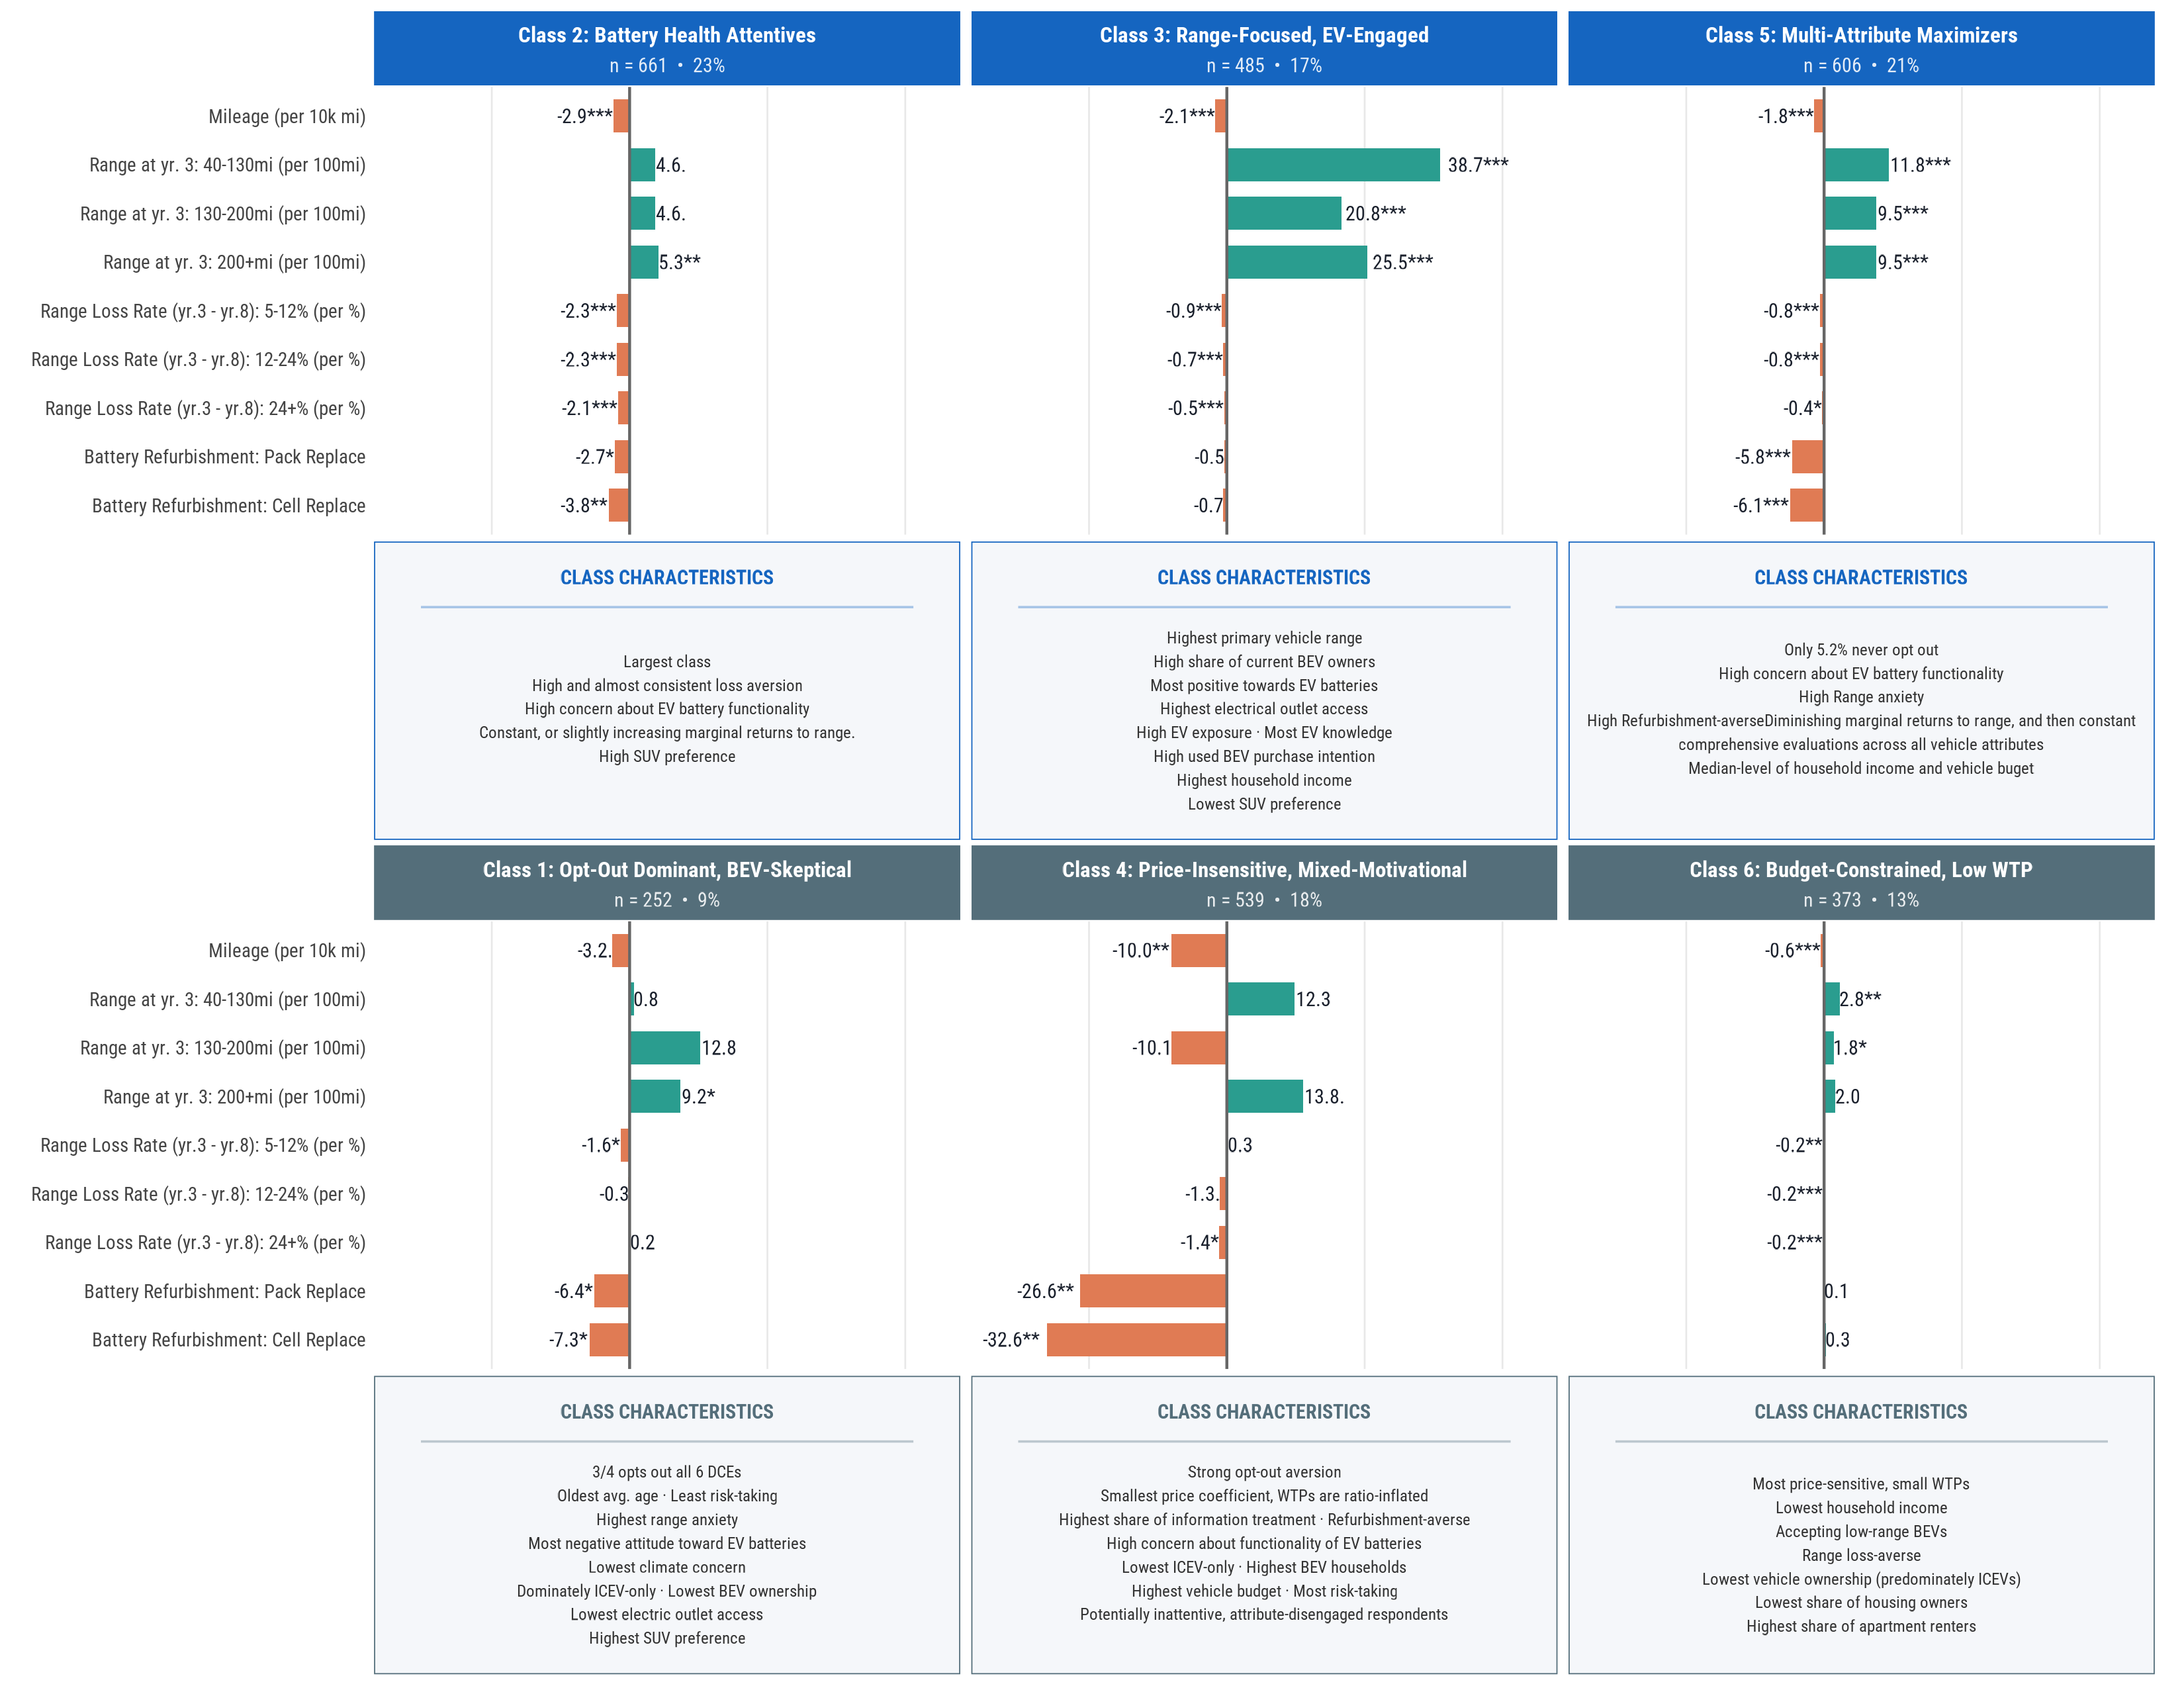
\includegraphics[width=0.88\linewidth, keepaspectratio]{../../code/output/model_output/battery_analysis/apollo/0_lc6_class_profiles_no_optout.png}
    \caption{WTP and class profile summary.}
    \label{fig:lc6_class_profiles}
\end{figure}
\end{landscape}





\end{document}
